\documentclass[10pt,a4paper]{article}
\usepackage[margin=2.2cm]{geometry}
\usepackage{fontspec}
\setmainfont{Libertinus Serif}
\setsansfont{IBM Plex Sans}
\setmonofont[Scale=0.86]{IBM Plex Mono}
\usepackage{microtype,graphicx,booktabs,tabularx,xcolor,float,fvextra,caption}
\usepackage[numbers,sort&compress]{natbib}
\usepackage[colorlinks,linkcolor=teal!70!black,citecolor=teal!70!black,urlcolor=teal!70!black]{hyperref}
\newfloat{listing}{tbp}{lol}\floatname{listing}{Listing}
\captionsetup{font=small,labelfont=bf}
\renewcommand{\tabularxcolumn}[1]{>{\raggedright\arraybackslash}p{#1}}
\setlength{\tabcolsep}{4pt}
\title{From Culture-Level Plans to Verified Robot Motions:\\ Reproducible and Auditable Experiments in a Robotic Laboratory Twin}
\author{[Author names and affiliations]}
\date{Preprint draft, generated 2026-10-17 \\ \small manifest \texttt{a8a39851a44328aa}}
\begin{document}
\maketitle
\begin{abstract}
Laboratory automation promises reproducible experiments. Yet an automated protocol is usually written at the level of devices and robot programs, so the scientific intent, its laboratory realization and the record of what happened are hard to separate, to check and to reproduce. We describe a pipeline in which an experiment is stated once, as a plan over the cultures: what is done to them, how they are observed and what becomes known. Everything else is derived from it: the experimental design by expected information gain, a partially ordered plan of laboratory action designators, a structured reactive controller in CRAM/RPL, 151 grounded robot and device steps, and 111 constraint-based motion specifications for Giskard. A machine-checked refinement proof shows that, under six stated assumptions about controllers, sensors and devices, every execution of the motion plan either realizes the culture plan while satisfying all stated safety, timing and contamination constraints, or is stopped by a monitor and ends in a failure handler whose guarantee holds. The derivation is recorded in a content-addressed manifest. A complete re-run reproduced all 47 outputs of its 12 stages identically; only wall-clock timing fields are excluded from the comparison. Execution produces a hash-chained audit trail that is itself reproducible: re-executing each of the 12 symbolic scenarios yields the identical chain head. We demonstrate the pipeline on a challenge–rescue organoid experiment in a physics-based digital twin of a two-arm robotic cell. The biology is a surrogate model and all biomedical parameters are illustrative. The paper itself is a build product of the pipeline.
\end{abstract}

\section{Introduction}\label{sec:intro}

Robotic laboratories can run experiments without interruption and record every action they take~\citep{king2009,williams2015,burger2020,abolhasani2023}. Reproducibility, however, needs more than automation~\citep{baker2016}. A protocol for a liquid handler and a plate-moving robot fixes \emph{how} an experiment is executed in one laboratory. It does not state \emph{what} the experiment does to the biological material, and it cannot be checked against that intent. When the laboratory changes (another robot, another incubator, a new safety rule), the protocol has to be rewritten, and nothing shows that the new protocol performs the same experiment.

We take the opposite route. The experiment is written once, at the level of the cultures: which culture is challenged, rescued, grown, observed, interpreted and analysed; which physical change each action causes; and which knowledge it produces. The plan says nothing about robots, devices, poses, safety rules, cleanliness or temperature control. Everything below it is derived and checked: the design, the laboratory plan, the controller, the robot and device steps, and the robot motions. The derivation is recorded so that anyone with the inputs can reproduce it. The execution is recorded so that anyone can verify it and re-execute it.

Contributions:

\begin{itemize}
  \item \textbf{A culture-level plan language} with physical and knowledge effects, built on entity-based designators. A partial order is derived from causal links, and the plan is independent of the laboratory: we show this over 13 laboratory variants (Section~\ref{sec:culture}).
  \item \textbf{An automatic refinement} from the culture plan to a least-cost design by expected information gain, to laboratory action designators with contracts and failure handlers, to a CRAM/RPL structured reactive controller, and to Giskard motion statecharts (Section~\ref{sec:refine}).
  \item \textbf{A machine-checked refinement proof} that the motion plan carries out the culture plan and satisfies every stated constraint, or fails safely, relative to explicit assumptions (Section~\ref{sec:proof}).
  \item \textbf{A reproducible derivation and a reproducible audit trail}: a content-addressed manifest that a re-run reproduces, and hash-chained trails whose chain heads are reproduced by re-execution (Section~\ref{sec:repro}).
  \item \textbf{The paper as a build product.} Every number, table, figure and listing in this paper is generated from the pipeline's outputs (manifest \texttt{a8a39851a44328aa}).
\end{itemize}

\begin{figure}[tbp]\centering
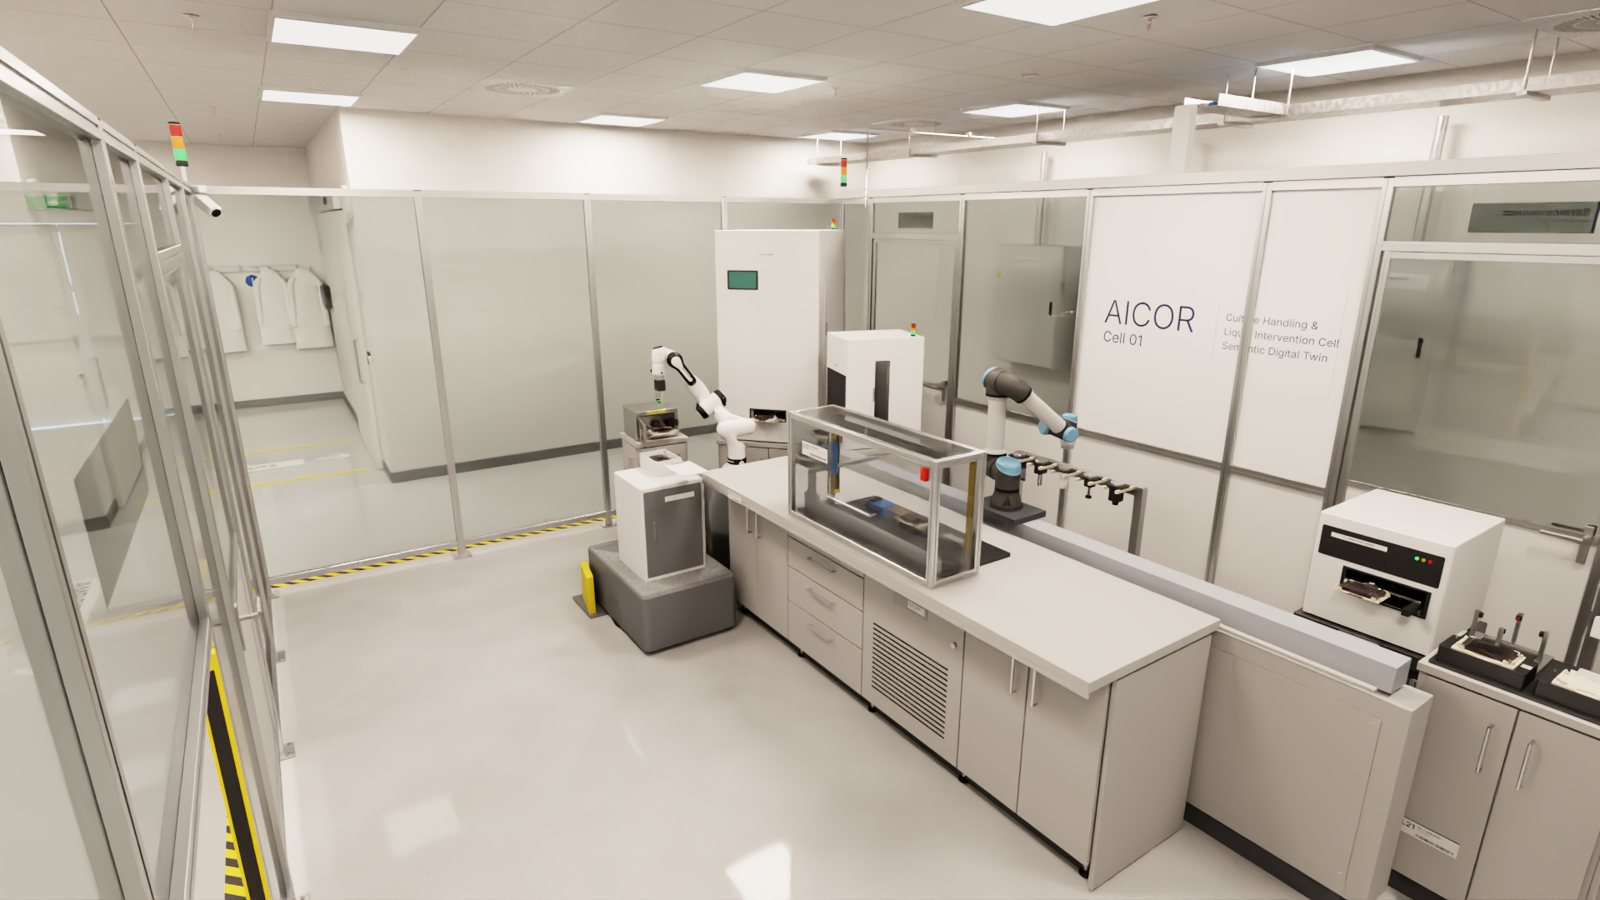
\includegraphics[width=\linewidth]{figures/cell.jpg}
\caption{Cell 01 in its semantic digital twin (Isaac Sim, path-traced): two arms, an incubator, a liquid handler in its enclosure, a bright-field imager, a tool rack and the handover nest. The experiment in this paper runs on this twin.}\label{fig:cell}
\end{figure}

\section{Related work}\label{sec:related}

\textbf{Robot scientists and self-driving laboratories.} Adam and Eve closed the loop from hypothesis to experiment in yeast genetics and drug screening~\citep{king2009,williams2015}. A mobile robot ran a chemistry search over a week of autonomous experiments~\citep{burger2020}. Self-driving laboratories are now common in chemistry and materials science~\citep{abolhasani2023}. These systems describe experiments at the level of the instruments. We add a level above the instruments and prove that the levels below realize it.

\textbf{Plan languages for robots.} RPL introduced concurrent reactive plans with failure handling and fluents~\citep{mcdermott1991}. Structured reactive controllers~\citep{beetz2001} and CRAM~\citep{beetz2010} made such plans the basis of everyday manipulation, using designators as symbolic descriptions that are resolved at run time, with knowledge supplied by KnowRob~\citep{tenorth2013}. Giskard specifies motions as constraint- and optimization-based tasks solved by model-predictive control~\citep{stelter2022}. We use these layers unchanged and add a culture level above them, together with proofs across the levels.

\textbf{Planning, design and verification.} The partial order of our plans follows least-commitment planning: causal links and threats~\citep{weld1994}. Designs are selected by expected information gain~\citep{lindley1956,chaloner1995}, and the least-cost plan is found with answer set programming~\citep{gebser2019}. Proof obligations are discharged by an SMT solver~\citep{demoura2008}. The refinement argument follows refinement mappings~\citep{abadi1991} and assume-guarantee contracts~\citep{benveniste2018}.

\textbf{Provenance and data integrity.} The audit trail is a hash chain in the sense of~\citep{haber1991}. Its entries follow W3C PROV~\citep{prov2013} and the ALCOA+ expectations for regulated records~\citep{fda2018}: attributable, legible, contemporaneous, original and accurate. The FAIR principles~\citep{wilkinson2016} motivate publishing the manifest together with the data.

\section{The experiment and the laboratory}\label{sec:setting}

The experiment asks which of three recovery models explains the efficacy of a rescue that follows a challenge: graded recovery (M1), a threshold (M2), or a protective effect (M3). Three cultures take part. The \emph{rescued} culture is challenged at 0 h and rescued later. The \emph{comparator} is challenged only. The \emph{control} is untreated. All three are imaged at 72 h, and the organoid radius is measured from the images. Doses are in arbitrary units (au). The culture dynamics, the imaging and the models are Cell 01's culture surrogate. The numbers are ILLUSTRATIVE and are not claims about any biological system.

Cell 01 (Fig.~\ref{fig:cell}) is a robotic cell for culture handling and liquid intervention. A seven-axis arm (R01) serves the incubator (L10) and the handover nest. A rail-mounted arm (R02) serves the liquid handler (L12), the imager (L17), a calibration and QC station (L21) and a quarantine station (H4), and changes tools at a rack. The cell is modelled as a semantic digital twin: an OWL ontology of the devices, seats, frames and safety rules, the component records of every device, and a USD scene that Isaac Sim simulates.

\section{The culture-level plan}\label{sec:culture}

A culture-level plan is a set of action designators over entity designators. An entity designator \texttt{(det sort ?var slot*)} describes an entity by its properties; it is resolved against a knowledge base and never names a device. Each action states its \emph{physical} effect on a culture and its \emph{knowledge} effect: what is recorded or inferred. Listing~\ref{lst:culture} shows the rescue. The goal of the plan is epistemic: the belief over the three models must have an expected information gain of at least 0.5 bit.

\begin{listing}[tbp]
\begin{Verbatim}[fontsize=\footnotesize,breaklines,frame=lines,framesep=2mm]
(an action ?c3
    (type rescuing)
    (culture ?cr)
    (substance ?rs)
    (dose 0.70 au)
    (at (culture-time 48 h))
    (requires (the experiment ?E (culture-time 48 h)))
    (physical (the culture ?cr (exposed-to ?rs 0.70 au))
              (the culture ?cr (recovery possible)))
    (knowledge (a record (of ?c3) (states ?cr ?rs 0.70 au 48 h))))
\end{Verbatim}
\caption{The rescue action of the culture plan (LDL). Times are culture times; the dose is ILLUSTRATIVE.}\label{lst:culture}
\end{listing}

The order is not written. It is derived from causal links: an action's requirement must be supported by an earlier action's physical or knowledge effect, or by the given state. The 12 actions have 13 causal links, and the partial order is their transitive reduction (Fig.~\ref{fig:poset}). Interpretation requires a known image scale. This requirement is marked \emph{establishable}: the plan states it, and the laboratory must establish it.

\begin{figure}[tbp]\centering
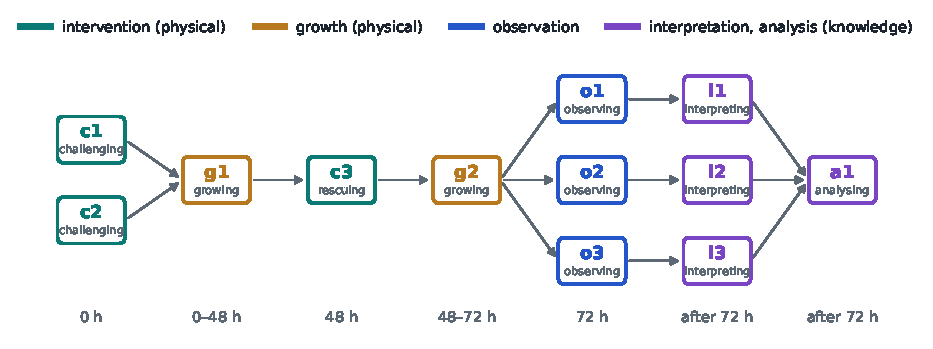
\includegraphics[width=\linewidth]{figures/poset.pdf}
\caption{The culture plan as a partial order (Hasse diagram of the derived causal order). Columns are culture-time phases.}\label{fig:poset}
\end{figure}

\textbf{Independence from the laboratory.} We checked the plan text against the realization vocabularies of the knowledge base: robots, devices, poses, seats, tools, safety rules, cleanliness and temperature. No term occurs in the plan. We then ran the whole refinement in 13 laboratory variants that change robots, devices, the layout, safety constraints, cleanliness and temperature profiles (appendix, Table~\ref{tab:labs}). The culture plan, its hash and its derived order are identical in all of them. Where a variant cannot realize the plan, the refusal names the missing capability. The plan itself is not changed.

\section{Refinement to robot motions}\label{sec:refine}

\begin{table}[tbp]\centering\small
\caption{The levels of the refinement. Each level is derived from the one above it and checked against it.}\label{tab:levels}
\begin{tabularx}{\linewidth}{lXlll}\toprule
\textbf{Level} & \textbf{States} & \textbf{Language} & \textbf{Derived by} & \textbf{Size} \\\midrule
Culture plan & what is done to the cultures, what becomes known & LDL (entity designators) & written & 12 actions \\
Design & doses, delay, replicates & EIG + ASP & nested Monte Carlo, clingo & 45 candidates \\
Lab plan & action designators with contracts and handlers & LDL & mapping, checked & 8 actions \\
Controller & structured reactive controller & CRAM/RPL (Lisp) & generated & 409 lines \\
Step plan & robot motions and device commands & kernel designators & clingo; kernel expansion & 151 steps \\
Motion plan & frames, constraints, monitors, cancels & giskardpy statecharts & generated & 111 motions \\\bottomrule
\end{tabularx}
\end{table}

\textbf{Design.} The free parameters of the culture plan (challenge dose, rescue delay, replicates) are chosen by expected information gain over a uniform prior on M1–M3. The gain is estimated by nested Monte Carlo on the surrogate (800 samples, seed 7). Of 45 candidates, 13 reach 0.5 bit (Fig.~\ref{fig:design}). An answer set program over the laboratory facts then selects the least-cost safe plan among them: challenge 0.85 au, rescue 0.7 au after 48 h, 1 replicate, EIG 0.5439 bit, at a cost of 9986 decisecond-equivalents.

\begin{figure}[tbp]\centering
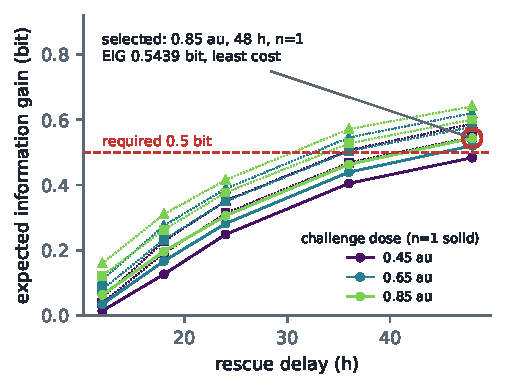
\includegraphics[width=0.62\linewidth]{figures/design.pdf}
\caption{Expected information gain of the candidate designs. The circle marks the selected design, the least-cost safe plan among the candidates that meet the requirement.}\label{fig:design}
\end{figure}

\textbf{Laboratory plan.} Each culture action is refined into a laboratory action designator (appendix, Table~\ref{tab:refine}). A laboratory action states what it \emph{requires}, what it \emph{prevents} and \emph{maintains} during a scope bounded by fluents, what it \emph{achieves}, its \emph{goal}, the failures it \emph{signals}, and an \emph{instrument role}: a slot that accepts the plate and a process that performs the action (Listing~\ref{lst:lab}). Instruments are resolved by capability. A device fills the role if it has the slot and can run the process. Process models of the devices list their faults, the monitors that detect them and the handlers that repair them. The checker verifies the causal links, resolves all 9 threats, resolves every instrument and verifies the guarantee of each of the 13 handlers: goal, goal-or-safe-state, safe state or containment.

\begin{listing}[tbp]
\begin{Verbatim}[fontsize=\footnotesize,breaklines,frame=lines,framesep=2mm]
(an action ?x3
    (type intervening)
    (into ?r)
    (substance ?rs)
    (dose 0.70 au)
    (at (culture-time 48 h)))
\end{Verbatim}
\caption{The laboratory action that refines the rescue. The instrument role, contracts and handlers come from the action type's contract.}\label{lst:lab}
\end{listing}

\textbf{Controller.} The laboratory plan is compiled into a CRAM/RPL structured reactive controller (Listing~\ref{lst:cram}). The partial order becomes \texttt{partial-\allowbreak{}order} constraints. \texttt{prevents} becomes a \texttt{with-\allowbreak{}policy} over a monitored fluent, bounded by a \texttt{scope}. \texttt{requires} becomes \texttt{ensure} with the epistemic grade the contract demands. Handlers become \texttt{with-\allowbreak{}failure-\allowbreak{}handling} clauses with retry counters.

\begin{listing}[tbp]
\begin{Verbatim}[fontsize=\footnotesize,breaklines,frame=lines,framesep=2mm]
(def-action-plan intervening ((into ?w) (substance ?s) (dose ?q) (at ?t))
  "Goal: (the well ?w (received ?s ?q)). Performed in: x1, x2, x3."
  (let* ((?self (current-action-designator))
         (?p (plate-of ?w))
         (?instrument (an instrument
                          (slot (a plate-slot (accepts ?p)))
                          (process (a process
                                       (type substance-transfer)
                                       (into ?w)
                                       (of ?s)
                                       (amount ?q))))))
    (with-retry-counters ((wrong-reagent-repairs 1) (tip-missing-or-dropped-repairs 1))
      (with-failure-handling
          ((dose-not-delivered (f)
             (case (failure-cause f)
               ;; perform again; guarantees goal-or-safe-state: holds
               (wrong_reagent (do-retry wrong-reagent-repairs
                                (achieve (some substance ?s (identity verified)))
                                (retry)))
               ;; perform again; guarantees goal-or-safe-state: holds
               (tip_missing_or_dropped (do-retry tip-missing-or-dropped-repairs (retry))))))
        (seq
          (ensure (the plate ?p (identity verified))
                  :grade (freshness fresh source observed)
                  :consequential t)
          (ensure (some substance ?s (identity verified))
                  :grade (freshness fresh source observed)
                  :consequential t)
          (ensure (the plate ?p (contamination none))
                  :grade (freshness fresh source inferred)
                  :consequential t)
          ;; supplied by a predecessor in the partial order
          (wait-for (holds (the plate ?p (culture-time ?t))))
          (with-policy (par
                         (prevent (holds (an event (type contamination-introduced) (of ?p)))
                                  contamination-suspected)
                         (scope ((holds (a portion ?u (of ?s) (drawn-for ?self)))
                                 (holds (the portion ?u (delivered true))))
                           (prevent (holds (a transfer (of ?u) (into (a well (of ?p) (not ?w)))))
                                    prevents-violated)))
            (perform (an action (type tending) (instrument ?instrument) (object ?p))))
          (check-goal (the well ?w (received ?s ?q)) dose-not-delivered))))))
\end{Verbatim}
\caption{Generated CRAM/RPL action plan for the intervening type (excerpt).}\label{lst:cram}
\end{listing}

\textbf{Steps.} The kernel expands the controller into grounded steps: 151 robot motions and device commands in 3 trips. The answer set program derives the same plan independently, and both agree step for step and second for second. The z3 validator proves executability, the safety rules (L12 airspace, environment before storage, calibration before imaging, interlocks, identity), the 600 s window outside the incubator, the realization of every dose and image, and least cost (10 negative controls).

\textbf{Motions.} Each robot step is refined into a giskardpy motion statechart (Listing~\ref{lst:giskard}). Goal frames are taken from the composed scene: seat frames, approach poses and well frames re-parented to the plate. A Cartesian task specifies the goal, velocity limits and level-keeping are weighted constraints, and collision avoidance is a constraint set. The quadratic program minimizes velocity and jerk over the horizon plus the weighted slacks. All 25 goal frames are reachable by inverse kinematics with joint margin. Because level-keeping and collision terms are soft, the generator adds monitors that cancel the motion when tilt, collision distance or duration exceeds its bound. This makes every soft constraint \emph{hold-or-cancel}.

\begin{listing}[tbp]
\begin{Verbatim}[fontsize=\footnotesize,breaklines,frame=lines,framesep=2mm]
def inserting(world, robot, seat, z, speed, tol, plate):
    root, tcp = body(world, robot["root"]), body(world, robot["tcp"])
    goal = tool_down(body(world, seat), z)
    done = PoseReached(root_link=root, tip_link=tcp, goal_pose=goal.to_homogeneous_matrix(),
                       position_threshold=tol, orientation_threshold=ORI_TOL)
    aux = [CartesianPoseStraight(root_link=root, tip_link=tcp, goal_pose=goal),
           CartesianPositionVelocityLimit(root_link=root, tip_link=tcp, max_linear_velocity=speed, weight=W_SPEED),
           allow_contact([body(world, j) for j in robot["finger_links"]], [plate])]
    return done, aux


def straight(world, robot, seat, z, speed, plate=None, contact=None):
    """lifting, placing, retracting: straight vertical motion of the TCP at a capped speed."""
    root, tcp = body(world, robot["root"]), body(world, robot["tcp"])
    done = CartesianPositionStraight(root_link=root, tip_link=tcp,
                                     goal_point=Point3(0.0, 0.0, z, reference_frame=body(world, seat)),
                                     reference_velocity=speed, threshold=POSE_TOL)
    aux = [CartesianPositionVelocityLimit(root_link=root, tip_link=tcp, max_linear_velocity=speed, weight=W_SPEED)]
    if plate is not None:
        aux.append(keep_level(world, plate))
    if contact is not None:
        aux.append(allow_contact(*contact))
    return done, aux
\end{Verbatim}
\caption{Generated Giskard phase for inserting the gripper at a seat (excerpt): the end monitor, the straight-line task, the speed limit and the permitted finger contact.}\label{lst:giskard}
\end{listing}

\section{Correctness of the refinement}\label{sec:proof}

\textbf{Theorem.} Under assumptions A1–A6 (Table~\ref{tab:assumptions}), every execution of the motion plan does one of two things. (i) It realizes the culture plan: every physical and knowledge effect, in the derived order, at 0, 48 and 72 h of culture time, with the control culture untreated, while interlocks, L12 airspace, identity, environment before storage, calibration before imaging, the 600 s window, contamination freedom, tool hygiene, plate level and collision distance all hold. (ii) Or a monitor stops it, and it ends in a failure handler whose guarantee holds.

The proof composes seven obligations along the refinement chain (Fig.~\ref{fig:chain}, Table~\ref{tab:obligations}). The step-level validator proves which doses, images and session times every execution produces. O2 maps them through the vessel map (rescued → A01, comparator → A02, control → A05) and shows with z3 that the negation of each culture-level obligation is unsatisfiable. O6 is where the soft optimization meets the logic. Each motion's end monitor implies its step's postcondition under A3. Each motion's timeout is 1.2 times its estimate, which is exactly the duration bound that the step-level timing proof assumes. A held plate's tilt and every collision distance cancel the motion when violated. O7 closes the failure branch: a cancellation raises a failure that propagates to a handler whose guarantee O3 verified.

\begin{figure}[tbp]\centering
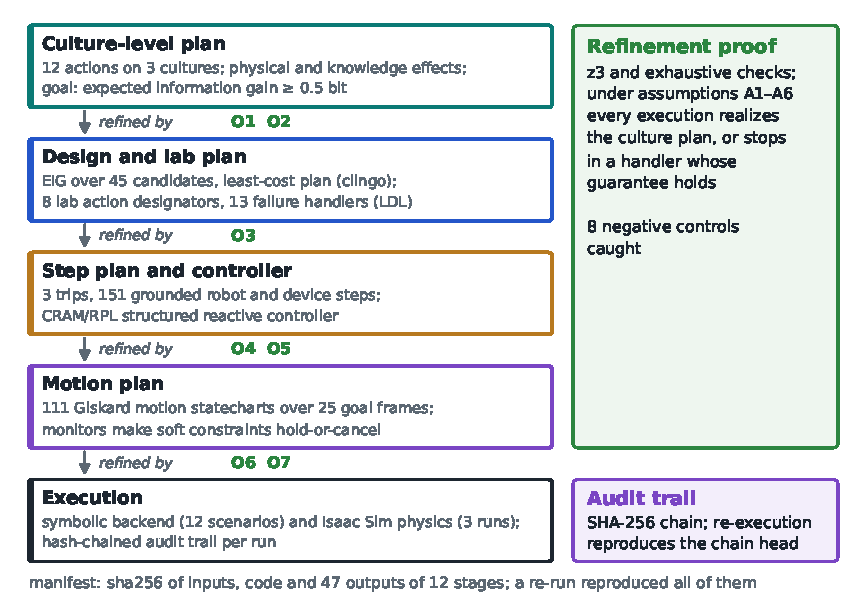
\includegraphics[width=0.92\linewidth]{figures/chain.pdf}
\caption{The refinement chain, the proof obligations O1–O7 on its links, and the records that make it reproducible.}\label{fig:chain}
\end{figure}

\begin{table}[tbp]\centering\small
\caption{Proof obligations and how they are discharged.}\label{tab:obligations}
\begin{tabularx}{\linewidth}{lXll}\toprule
\textbf{} & \textbf{Obligation} & \textbf{Discharged by} & \textbf{Result} \\\midrule
O1 & culture plan well formed (supported, acyclic) & causal-link analysis & 13 links \\
O2 & step-level events entail every culture effect, the order and the culture prevents & z3 (negation UNSAT) & 14/14 \\
O3 & lab plan: links, threats, instruments, handler guarantees & LDL checker & threats 9/9, guarantees 13/13 \\
O4 & step plan: executability, safety, time, realization, gain, least cost & z3 (V1–V5) & 7/7 theorems \\
O5 & no plate-handling tool touches the culture & z3 & holds \\
O6 & each motion refines its step; end monitor implies the postcondition; soft parts hold-or-cancel & exhaustive check & 111/111 motions \\
O7 & every cancellation reaches a handler with a verified guarantee & exhaustive check & 13 failure types \\\bottomrule
\end{tabularx}
\end{table}

\begin{table}[tbp]\centering\small
\caption{Assumptions of the theorem and how each is covered.}\label{tab:assumptions}
\begin{tabularx}{\linewidth}{lXl}\toprule
\textbf{} & \textbf{Assumption} & \textbf{Covered by} \\\midrule
A1 & a motion statechart ends only through EndMotion (its end monitor true) or CancelMotion. & library semantics \\
A2 & PoseReached, LocalMinimumReached with the grasp check, VectorsAligned, the collision distance monitors, the simulation clock, the barcode read, the seat sensors and the device monitors observe correctly. & assumed; 2 fault kinds only partly detected \\
A3 & a TCP within 0.4 mm / 0.2 deg of a seat's grasp or release pose has the plate in that seat (the nest guides capture it); within 5 mm of an approach pose it is at that approach pose (free-space waypoint). & ILLUSTRATIVE capture (2 mm) \\
A4 & grasp\_confirmed, lifted, seating). & monitored at run time \\
A5 & dose\_well delivers within its tolerance when its monitors pass; image\_well yields an image when calibration and focus monitors pass; L10 holds the environment profile while the plate is stored. & component contracts, monitored \\
A6 & the goal frames are the ones the scene defines (rsa/motion\_frames.py), and each is reachable (checked).  & checked (25/25) \\\bottomrule
\end{tabularx}
\end{table}

\textbf{Negative controls.} To show that the checks are not vacuous, each of 8 mutations must make an obligation fail: a swapped vessel map, a dosed control, a missing control image, a contaminating tool, a held motion without its tilt monitor, a timeout beyond the timing bound, a motion that does not refine its step, and the validator's own mutated plans. All are caught (Table~\ref{tab:negative}).

\section{Reproducible derivation and audit}\label{sec:repro}

\textbf{Manifest.} The pipeline runs in 12 stages, from the design to the protocol (Table~\ref{tab:repro}). For each stage the manifest records the command, the sha256 of the code it ran and the sha256 of every file it wrote. The inputs (culture plan, registry, ontology ABox, answer set program, scene, surrogate code, duration traces and the recorded physics runs) and the tool versions are recorded once. JSON outputs are hashed in canonical form without the wall-clock fields (\texttt{ground\_s}, \texttt{solve\_s}, \texttt{validator\_wall\_s}, \texttt{wall\_s}). Nothing else is excluded. The manifest hash identifies the whole derivation: \texttt{a8a39851a44328aac152ee46629decd9cddc691b1e8c2b835c422bba7cd32659}.

\textbf{Reproduction.} A second complete run, which also recomputes the Monte Carlo estimates from scratch, produced the same manifest hash. All 47 of 47 outputs are identical, including the plan, the proofs, the controller, the generated Giskard module and all audit trails.

\begin{table}[tbp]\centering\small
\caption{Stages of the pipeline and the result of the reproduction run.}\label{tab:repro}
\begin{tabularx}{\linewidth}{lXrr}\toprule
\textbf{Stage} & \textbf{Derives} & \textbf{Outputs} & \textbf{Identical} \\\midrule
design & EIG over the competing recovery models; least-cost safe plan meeting 0.5 bit (clingo) & 4 & 4 \\
step-proof & SMT validation of the plan: executability, safety, time, realization, gain, least cost (z3) & 1 & 1 \\
culture & culture plan: causal order, surrogate execution, mapping to the lab, transport and tending feasibility & 1 & 1 \\
lab-plan & lab action designators: order, threats, instruments, process models, handlers, guarantees, KPIs & 1 & 1 \\
controller & CRAM/RPL structured reactive controller (Lisp) & 3 & 3 \\
execution & kernel execution on the symbolic backend: 12 scenarios, audit trails, critic, tamper test, competency questions & 26 & 26 \\
grounding & cultures on plates, trips, device programs, monitors, reactions & 1 & 1 \\
frames & goal frames from the scene; reachability (IK) of every goal & 1 & 1 \\
motions & Giskard motion statecharts: frames, constraints, monitors, cancels & 3 & 3 \\
independence & the culture plan in 13 lab variants & 1 & 1 \\
refinement-proof & motion plan refines the culture plan (O1-O7, negative controls) & 2 & 2 \\
protocol & experimentation plan (protocol) and audit certificate: chains, tamper test, re-execution of every symbolic trail & 3 & 3 \\\bottomrule
\end{tabularx}
\end{table}

\textbf{Audit trail.} Every lifecycle transition of every designator (open, grounded, accepted, executing, executed, failed, repaired) is one entry of a SHA-256 hash chain. The entry hash covers the previous hash and the canonical JSON of the entry (Listing~\ref{lst:audit}). The executor writes the entries, not the plan, so a plan cannot skip them. Entries record the agent, the software (kernel, knowledge base, registry hash, backend), the simulated time, bindings and resolutions with their grounds, constraint verdicts in two columns (realization and validity), monitors, and evidence with its own sha256.

\begin{listing}[tbp]
\begin{Verbatim}[fontsize=\footnotesize,breaklines,frame=lines,framesep=2mm]
{
  "seq": 86,
  "t_sim": 156.1,
  "designator": "d0039-dispense",
  "parent": "d0036-dose",
  "kind": "command",
  "category": "dispense",
  "transition": "executed",
  "agent": "l12",
  "software": {"kernel": "rsa-kernel/0.1", "kb": "facts_g050+nominal", "registry": "5d901b7f8087...
  "term": ["cmd", "l12", ["dispense", "https___aicor_example_okf_sdt_lab1_world_experimentalworl...
  "monitors": [{"name": "well_binding", "passed": true, "observation": "P17/A01"}, {"name": "dis...
  "constraints": [{"id": "l12_airspace_clear", "column": "realization", "verdict": "ENFORCED", "...
  "evidence": [  // 10 items, each with its own sha256
    {"kind": "plate", "value": "P17", "sha256": "6f418d76902ea3669355d6f0f3abf4387fe78c83d8b...,
    {"kind": "well", "value": "A01", "sha256": "3b1d4717064134258d9fc1cdb2a8055c242348548558...,
    {"kind": "reagent", "value": "challenge", "sha256": "d0303e386ced87e527d925fae2b47bbbf40...,
    ...],
  "prev": "32dddeae06c3eed2acaa64bf9e9f446a834a8539ff4e35f1ec28bf0ded3ce3b9",
  "hash": "e890f45744b3ada383becbcd869882c65acd04239017d16b015f077ee6d9c739",
}
\end{Verbatim}
\caption{An audit entry (abbreviated; ... marks truncation): a dispense command executed by L12, with its monitors, constraint verdicts and hashed evidence.}\label{lst:audit}
\end{listing}

\textbf{Verification.} For all 15 trails the chain is intact. Changing a single value is detected at the changed entry. Re-executing each of the 12 symbolic scenarios in a fresh directory reproduces its trail exactly, chain head included (12/12). A trail is therefore more than a tamper-evident record: it is a reproducible one, and its head hash commits to the whole execution. The 52 competency questions of the kernel are audit questions: what was done, why, how, under which constraints, with which evidence, and what would have happened if. All 52 are answered correctly from the trails alone.

\section{Execution}\label{sec:exec}

Table~\ref{tab:scenarios} lists the executions. On the symbolic backend, 12 scenarios inject knowledge errors, faults and workflow errors: lapsed calibration, a lost tip, a swapped plate identity, a slow tool changer, a swapped or incapable imager, an unbound rescue, a dropped control, contamination and an incomplete component record. Every scenario ends as specified before it was run. The ends are executed, executed after a local repair, escalated to a human, or refused before anything moved.

\begin{table}[tbp]\centering\small
\caption{Executions. R | V: realization and validity columns of the verdict. 'As specified': the end and the verdict match the expectation written before the run.}\label{tab:scenarios}
\begin{tabularx}{\linewidth}{lllllll}\toprule
\textbf{Scenario} & \textbf{Backend} & \textbf{End} & \textbf{R | V} & \textbf{Repairs} & \textbf{Entries} & \textbf{As specified} \\\midrule
nominal & symbolic & executed & ok | ok & – & 498 & yes \\
calibration lapsed & symbolic & executed & ok | ok & image & 569 & yes \\
card incomplete & symbolic & abstained & – | – & – & 3 & yes \\
contamination & symbolic & abstained & – | – & – & 3 & yes \\
control dropped & symbolic & abstained & – | – & – & 3 & yes \\
identity swap & symbolic & escalated & – | – & retrieve & 224 & yes \\
imager incapable & symbolic & abstained & – | – & – & 3 & yes \\
imager swapped & symbolic & executed & ok | – & – & 498 & yes \\
rescue unbound & symbolic & abstained & – | – & – & 3 & yes \\
tip lost & symbolic & executed & ok | ok & dose & 501 & yes \\
tool changer slow & symbolic & escalated & – | – & run\_session & 266 & yes \\
uncalibrated known & symbolic & executed & ok | ok & – & 504 & yes \\
nominal & Isaac Sim & executed & ok | ok & – & 498 & yes \\
calibration lapsed & Isaac Sim & escalated & – | – & run\_session, image, image & 562 & NO \\
identity swap & Isaac Sim & escalated & – | – & retrieve & 56 & yes \\\bottomrule
\end{tabularx}
\end{table}

In Isaac Sim, the nominal run executes all three trips (Fig.~\ref{fig:gantt}). The physics-timed trips deviate from the planned durations by +2.3 \%, -12.6 \%, -19.1 \%, which lies within the ±20 \% that the timing proof assumes, and every trip stays inside the 600 s window. The identity-swap run detects the wrong plate at the incubator's barcode read, quarantines it and escalates, as specified. The lapsed-calibration run does \textbf{not} end as specified. The calibration repair worked: the imager refused, the plate was set aside, the station recalibrated and the measurement was re-planned. But the comparator well then failed the focus check twice, and the session escalated. The images after the reload show a lateral shift of about 93 µm that the seat sensors did not register. The kernel's refocus repair cannot change the outcome, because the imager autofocuses on every image anyway. We report this failure because it marks the boundary of the proof: plate misseating on the imager is one of the two partly detected faults (Section~\ref{sec:limits}).

\begin{figure}[tbp]\centering
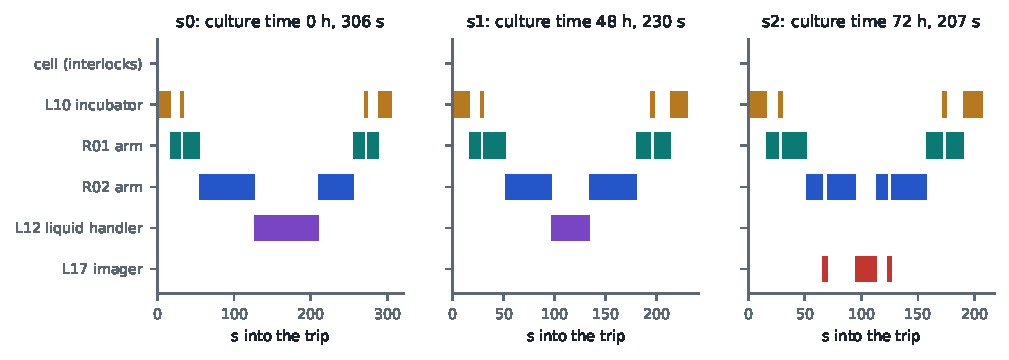
\includegraphics[width=\linewidth]{figures/gantt.pdf}
\caption{The nominal run in Isaac Sim: what each agent does during each trip (physics-timed leaves of the audit trail).}\label{fig:gantt}
\end{figure}

\textbf{Knowledge.} Executed on the surrogate, the analysis moves the belief from uniform to M1 0.68, M2 0.15, M3 0.17. The realized information gain is 0.357 bit, below the expected 0.544 bit. The plan's goal is an \emph{expected} gain, which a single outcome need not reach. A sequential design conditions the next plan on this posterior.

\section{Limitations}\label{sec:limits}

\begin{itemize}
  \item \textbf{No wet-lab execution.} The experiment ran on a digital twin with a surrogate culture model. All biomedical parameters are ILLUSTRATIVE.
  \item \textbf{Relative correctness.} The theorem holds relative to A1–A6. It does not prove progress: a motion may be cancelled rather than complete. 6 of the 27 fault instances in the process models are only partly detected (well misregistration at the liquid handler, plate misseating at the imager). An undetected occurrence lies outside both branches of the theorem.
  \item \textbf{Physics.} Compliant insertion into the nests has no Giskard counterpart yet. The 2 mm capture and the 2° tilt bound are ILLUSTRATIVE. The generated Giskard module has been checked against the giskardpy sources but not executed, because no semantic digital twin world of Cell 01 is loaded into Giskard. Collisions of R02 are not checked offline.
  \item \textbf{Reproduction scope.} The reproduction ran on the same machine with the same environment. The Isaac Sim runs are recorded inputs: their chains are verified, but they were not re-executed, and physics simulation on a GPU is not expected to be bit-reproducible.
  \item \textbf{References and authorship.} The reference list was compiled without database access and must be checked before submission.
\end{itemize}

\section{Conclusion}\label{sec:conclusion}

An experiment can be stated at the level at which a scientist thinks about it, as a plan over cultures and knowledge, and still be carried out by robots under proofs that connect the two levels. The derivation and the execution can both be reproduced from content-addressed records. The proof is only as strong as its assumptions, and the experiment in this paper found where they are weakest: in how plates sit in their nests. The next steps are to execute the motion statecharts in Giskard against the semantic digital twin, to close the two detection gaps with monitors that make misseating observable, and to run the same culture plan in a wet laboratory.

\paragraph{Code and data availability.} All inputs, code and outputs are in the project repository (\texttt{rsa/}, \texttt{okf/lab-\allowbreak{}automation-\allowbreak{}twin/}). \texttt{python -\allowbreak{}m rsa.reproduce} re-runs the derivation, and \texttt{python -\allowbreak{}m rsa.reproduce -\allowbreak{}-\allowbreak{}verify} compares the result with the manifest \texttt{a8a39851a44328aa}. \texttt{python -\allowbreak{}m rsa.protocol} writes the experimentation plan and the audit certificate. \texttt{python paper/build\_paper.py} rebuilds this paper.

\paragraph{Use of AI assistance.} Code, analyses and the text of this paper were produced with an AI coding assistant (Claude, Anthropic) under the authors' direction. The authors checked the results and are responsible for the content. [Authors: adapt this statement to the venue's policy.]

\bibliographystyle{unsrtnat}
\bibliography{refs}
\appendix

\section{Experimentation plan (generated)}\label{sec:protocol}

The plan below is generated from the pipeline's outputs (\texttt{rsa/out/repro/protocol.md}). It is the protocol a laboratory would run, bound to the derivation by the input digest \texttt{d514d47b1ad1b075}.

\begin{table}[tbp]\centering\small
\caption{Trips: culture time, device, material, number of steps, planned and physics-timed duration.}\label{tab:sessions}
\begin{tabularx}{\linewidth}{lllXrrr}\toprule
\textbf{Session} & \textbf{Culture time} & \textbf{Device} & \textbf{Material} & \textbf{Steps} & \textbf{Planned (s)} & \textbf{Isaac (s)} \\\midrule
s0 & 0 h & L12 & dose A01 challenge 0.85 au; dose A02 challenge 0.85 au & 52 & 298.9 & 305.7 \\
s1 & 48 h & L12 & dose A01 rescue 0.70 au & 48 & 263.3 & 230.1 \\
s2 & 72 h & L17 & image A01; image A02; image A05 & 51 & 256.4 & 207.3 \\\bottomrule
\end{tabularx}
\end{table}

\begin{table}[tbp]\centering\small
\caption{Refinement of the culture actions into laboratory actions, processes and devices (computations run in the culture digital twin).}\label{tab:refine}
\begin{tabularx}{\linewidth}{lllX}\toprule
\textbf{Culture action} & \textbf{Lab action} & \textbf{Process} & \textbf{Realized by} \\\midrule
?c1 challenging & ?x1 intervening & substance-transfer & L12 \\
?c2 challenging & ?x2 intervening & substance-transfer & L12 \\
?g1 growing & ?w1 incubating & incubation & L10 \\
?c3 rescuing & ?x3 intervening & substance-transfer & L12 \\
?g2 growing & ?w2 incubating & incubation & L10 \\
?o1 observing & ?m1 measuring & imaging & L17 \\
?o2 observing & ?m2 measuring & imaging & L17 \\
?o3 observing & ?m3 measuring & imaging & L17 \\
?i1 interpreting &  computation &  & culture SDT image analysis (twin/culture/optics.analyse): radius from the calibrated pixel size \\
?i2 interpreting &  computation &  & culture SDT image analysis (twin/culture/optics.analyse): radius from the calibrated pixel size \\
?i3 interpreting &  computation &  & culture SDT image analysis (twin/culture/optics.analyse): radius from the calibrated pixel size \\
?a1 analysing &  computation &  & posterior over M1-M3 (twin/culture/eig.posterior\_over\_models) on the rescued - comparator radius \\\bottomrule
\end{tabularx}
\end{table}

\begin{table}[tbp]\centering\small
\caption{Failure handlers of the experiment with their guarantees.}\label{tab:handlers}
\begin{tabularx}{\linewidth}{lX}\toprule
\textbf{Failure} & \textbf{Handler (LDL)} \\\midrule
identity-mismatch & (on (a failure (type identity-mismatch)) (do (an action (type quarantining) (material (the plate (identity mismatched))))) (then escalate) (guarantees safe-state contained)) \\
measurement-invalid & (on (a failure (type measurement-invalid) (cause calibration\_expired)) (do (re-establish (an instrument (function imaging) (calibration current)))) (then replan) (else escalate) (guarantees goal-or-safe-state)) \\
measurement-invalid & (on (a failure (type measurement-invalid) (cause out\_of\_focus)) (do (re-establish (the plate ?p (seated true)))) (then (retry (max 1))) (else escalate) (guarantees goal-or-safe-state)) \\
measurement-invalid & (on (a failure (type measurement-invalid) (cause plate\_misseated)) (do (re-establish (the plate ?p (seated true)))) (then (retry (max 1))) (else escalate) (guarantees goal-or-safe-state)) \\
validity-effect-unachievable & (on (a failure (type validity-effect-unachievable)) (then escalate) (guarantees safe-state)) \\
dose-not-delivered & (on (a failure (type dose-not-delivered) (cause wrong\_reagent)) (do (re-establish (some substance ?s (identity verified)))) (then (retry (max 1))) (else escalate) (guarantees goal-or-safe-state)) \\
dose-not-delivered & (on (a failure (type dose-not-delivered) (cause tip\_missing\_or\_dropped)) (then (retry (max 1))) (else escalate) (guarantees goal-or-safe-state)) \\
dose-not-delivered & (on (a failure (type dose-not-delivered) (cause clog\_or\_air\_aspiration)) (then escalate) (guarantees safe-state)) \\
dose-not-delivered & (on (a failure (type dose-not-delivered) (cause well\_misregistration)) (do (an action (type quarantining) (material ?p))) (then escalate) (guarantees safe-state contained)) \\
contamination-suspected & (on (a failure (type contamination-suspected)) (do (an action (type quarantining) (material ?p))) (then escalate) (guarantees safe-state contained)) \\
environment-excursion & (on (a failure (type environment-excursion)) (do (restore (the plate ?p (in ?env)))) (then escalate) (guarantees safe-state)) \\
containment-breach & (on (a failure (type containment-breach)) (then escalate) (guarantees safe-state)) \\
prevents-violated & (on (a failure (type prevents-violated)) (do (restore (the plate ?p (in ?env)))) (then escalate) (guarantees safe-state)) \\\bottomrule
\end{tabularx}
\end{table}

\begin{table}[tbp]\centering\small
\caption{The culture plan in the laboratory variants: outcome and the hash of the culture plan.}\label{tab:labs}
\begin{tabularx}{\linewidth}{Xlll}\toprule
\textbf{Lab variant} & \textbf{Dimension} & \textbf{Outcome} & \textbf{Culture plan} \\\midrule
Cell 01 as built (layout P1) & (reference) & realized & a5e27614c98a \\
one rail robot serves every station (no R01, no handover) & robots & realized & a5e27614c98a \\
R02 keeps its plate tool coupled between trips & robots & realized & a5e27614c98a \\
R01 and R02 hand the plate over in the plate hotel L09, not a handover nest & lab setup & realized & a5e27614c98a \\
the imager replaced by a capability-matched model without a validated binding & devices & realized, result not valid evidence (NR3) & a5e27614c98a \\
the imager replaced by another model with a validated binding for the readout & devices & realized & a5e27614c98a \\
the liquid handler replaced by another model with the same capabilities & devices & realized & a5e27614c98a \\
the lab allows the plate only 300 s outside the incubator & safety constraints & refused before anything moved & a5e27614c98a \\
the enclosure interlocks are open & safety constraints & refused before anything moved & a5e27614c98a \\
contamination is suspected on the plate & cleanliness & refused before anything moved & a5e27614c98a \\
the lab classes the plate tool T01 as touching the culture & cleanliness & refused before anything moved & a5e27614c98a \\
the incubator keeps a different environment profile than culture-standard & temperature control & refused at mapping & a5e27614c98a \\
the imager's calibration is not current & calibration & realized & a5e27614c98a \\\bottomrule
\end{tabularx}
\end{table}

\begin{table}[tbp]\centering\small
\caption{Negative controls of the refinement proof.}\label{tab:negative}
\begin{tabularx}{\linewidth}{Xl}\toprule
\textbf{Mutation} & \textbf{Caught} \\\midrule
vessel map swaps rescued and comparator & yes \\
the control well A05 is also dosed & yes \\
the control well is not imaged & yes \\
the plate tool T01 touches the culture & yes \\
one held motion without the tilt cancel & yes \\
one motion's timeout beyond V3's bound (1.5 x) & yes \\
a motion that does not refine its step & yes \\
step level: the validator's own 10 mutated plans & yes \\\bottomrule
\end{tabularx}
\end{table}

\end{document}
